\documentclass[12pt]{article}
\usepackage[margin=0cm, paperwidth=16cm,paperheight=15cm]{geometry}
\usepackage[utf8]{inputenc}
\usepackage{csquotes}
\usepackage{graphicx}
\usepackage{subfigure}
\usepackage{amssymb,amsfonts,amsmath}
\usepackage{url}
\usepackage{booktabs, multicol, multirow}
\usepackage[round,sort,comma,numbers]{natbib}

\begin{document}

\begin{figure}

\begin{center}

\subfigure[]{
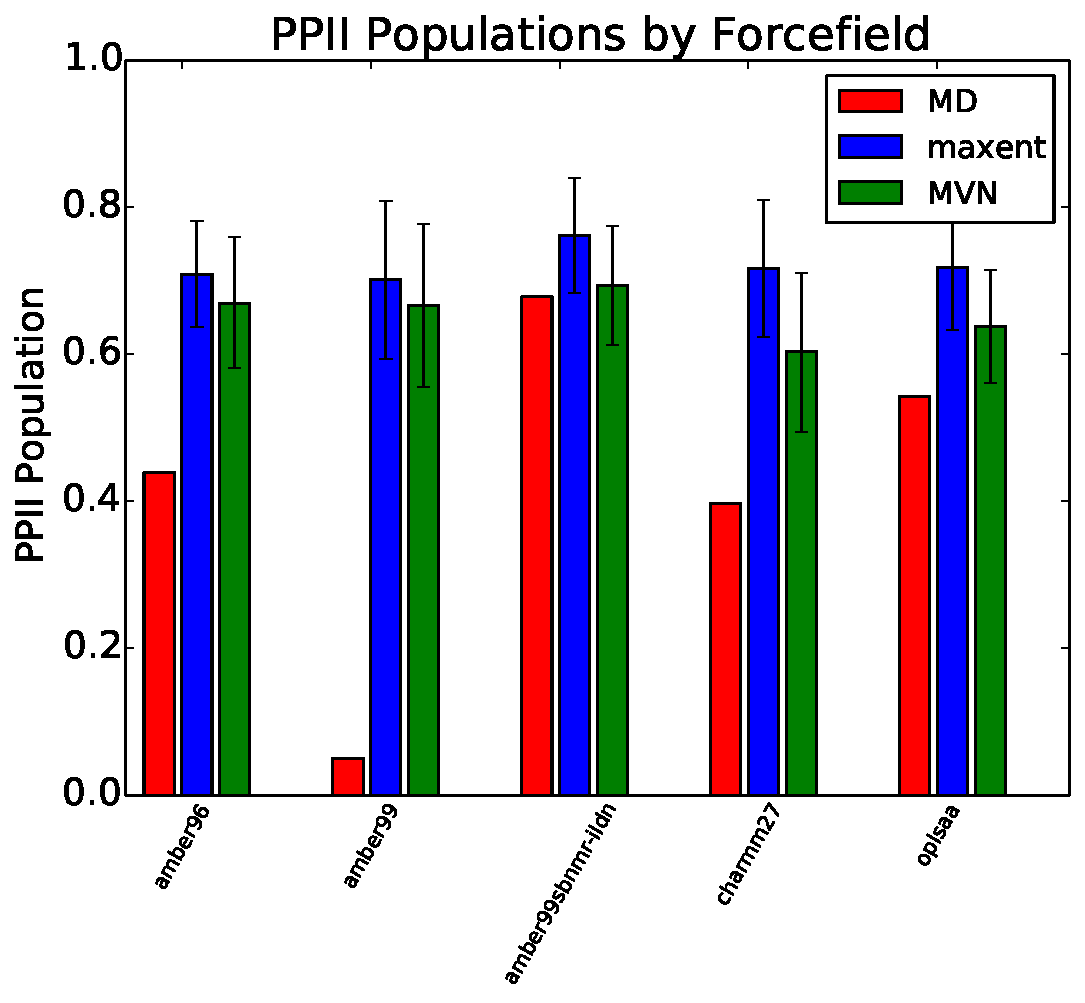
\includegraphics[width=7.5cm]{../figures/state_0_by_forcefield_priors.pdf}
}

\subfigure[]{
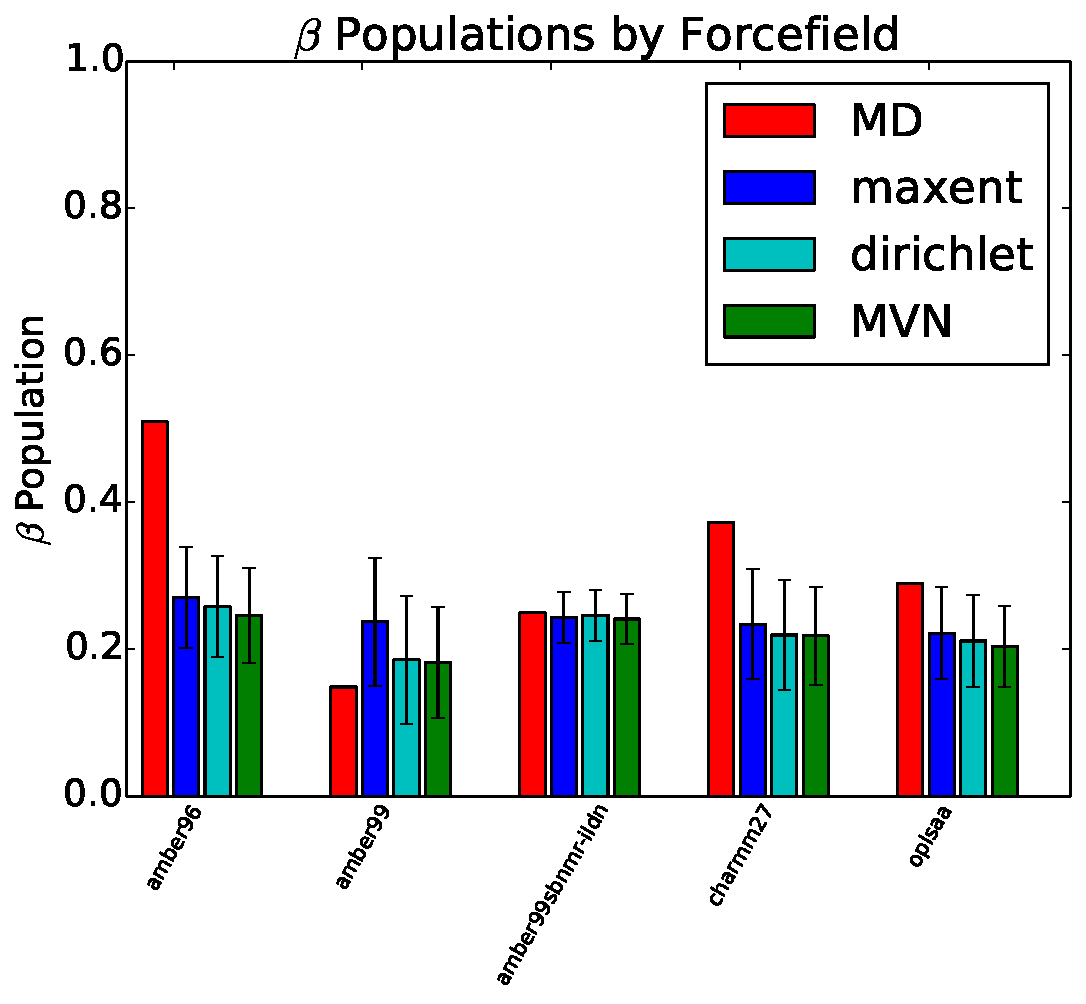
\includegraphics[width=7.5cm]{../figures/state_1_by_forcefield_priors.pdf}
}
\subfigure[]{
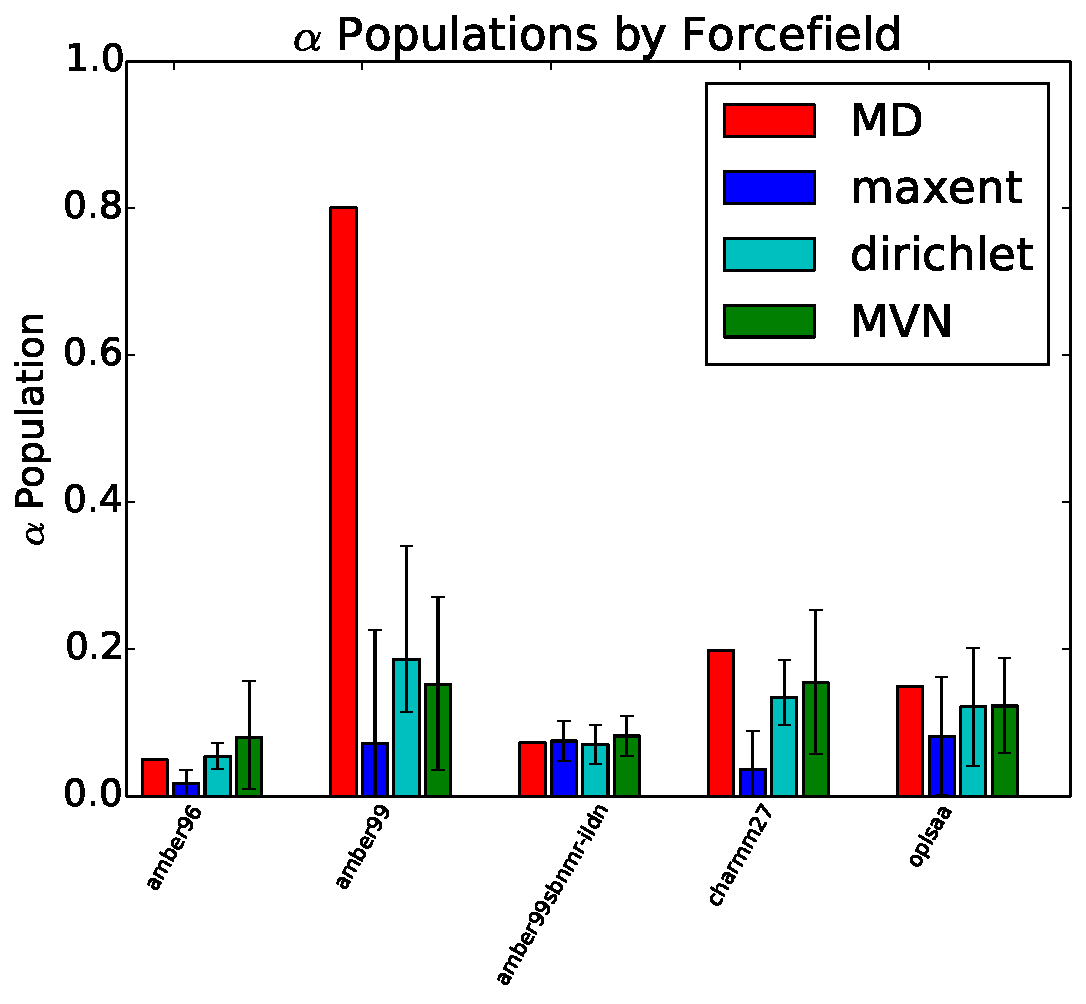
\includegraphics[width=7.5cm]{../figures/state_2_by_forcefield_priors.pdf}
}
\caption{
MD and BELT (maxent, Dirichlet, and MVN priors) conformational propensities (for central alanine residue) in each force field.  
}

\end{center}

\end{figure}

\end{document}
